\documentclass[xcolor=table]{beamer}
%\usepackage{beamerthemeSingapore}
%\usepackage{beamerthemeSingapore}
\usetheme{Singapore2}
\definecolor{themeColor}{RGB}{25,103,170}
\usecolortheme[named=themeColor]{structure}
\usepackage{microtype}
\usepackage{xspace}
\usepackage{grffile} %fix silly extension problems in graphics
%%%
\setbeamertemplate{navigation symbols}{} 
\usepackage{textcomp} %tilde
\usepackage{array} %M in tabulars



%http://tex.stackexchange.com/questions/65583/grey-not-black-shadow-box

\usepackage{tikz} 
\usetikzlibrary{shadows.blur}
\tikzset{
	every overlay node/.style={
		anchor=north west,
	},
}
% Usage:
% \tikzoverlay at (-1cm,-5cm) {content};
% or
% \tikzoverlay[text width=5cm] at (-1cm,-5cm) {content};
\def\tikzoverlay{%
	\tikz[baseline,overlay]\node[every overlay node]
}%


%http://tex.stackexchange.com/questions/40561/table-with-multiple-lines-in-some-cells
\newcommand{\thead}[2][.75in]{%
	\vbox{\hsize#1\baselineskip11pt\centering\vspace*{3pt}#2\par}}
	\arrayrulecolor{darkBorderColor}
	\rowcolors{1}{row1}{row2}

\colorlet{borderColor}{cyan!30!white!90!black!70}
\colorlet{darkBorderColor}{cyan!30!white!70!black!90}
\colorlet{headerColor}{cyan!20!white!90!black!70}
\colorlet{row1}{cyan!20!white!90!black!30}
\colorlet{row2}{cyan!20!white!50!black!30}

\colorlet{ShadowColor}{borderColor}
\colorlet{ShadowColor2}{darkBorderColor}

\title{\LARGE Introduction to command line}%\\\vspace{-.075in} analyzed by RNA-Seq\vspace{-.3in}}
\author{\vspace{-.2in}Scott Sherrill-Mix\vspace{-.4in}}
\date{\today\vspace{-.5in}}
\begin{document}
{
\frame[plain]{\vspace{-.3in}\titlepage}
}

\section{Intro}
\section{Command line}
\framedgraphic{What is command line?}{im/command.png}
\begin{frame}{Command line history}
\begin{center}
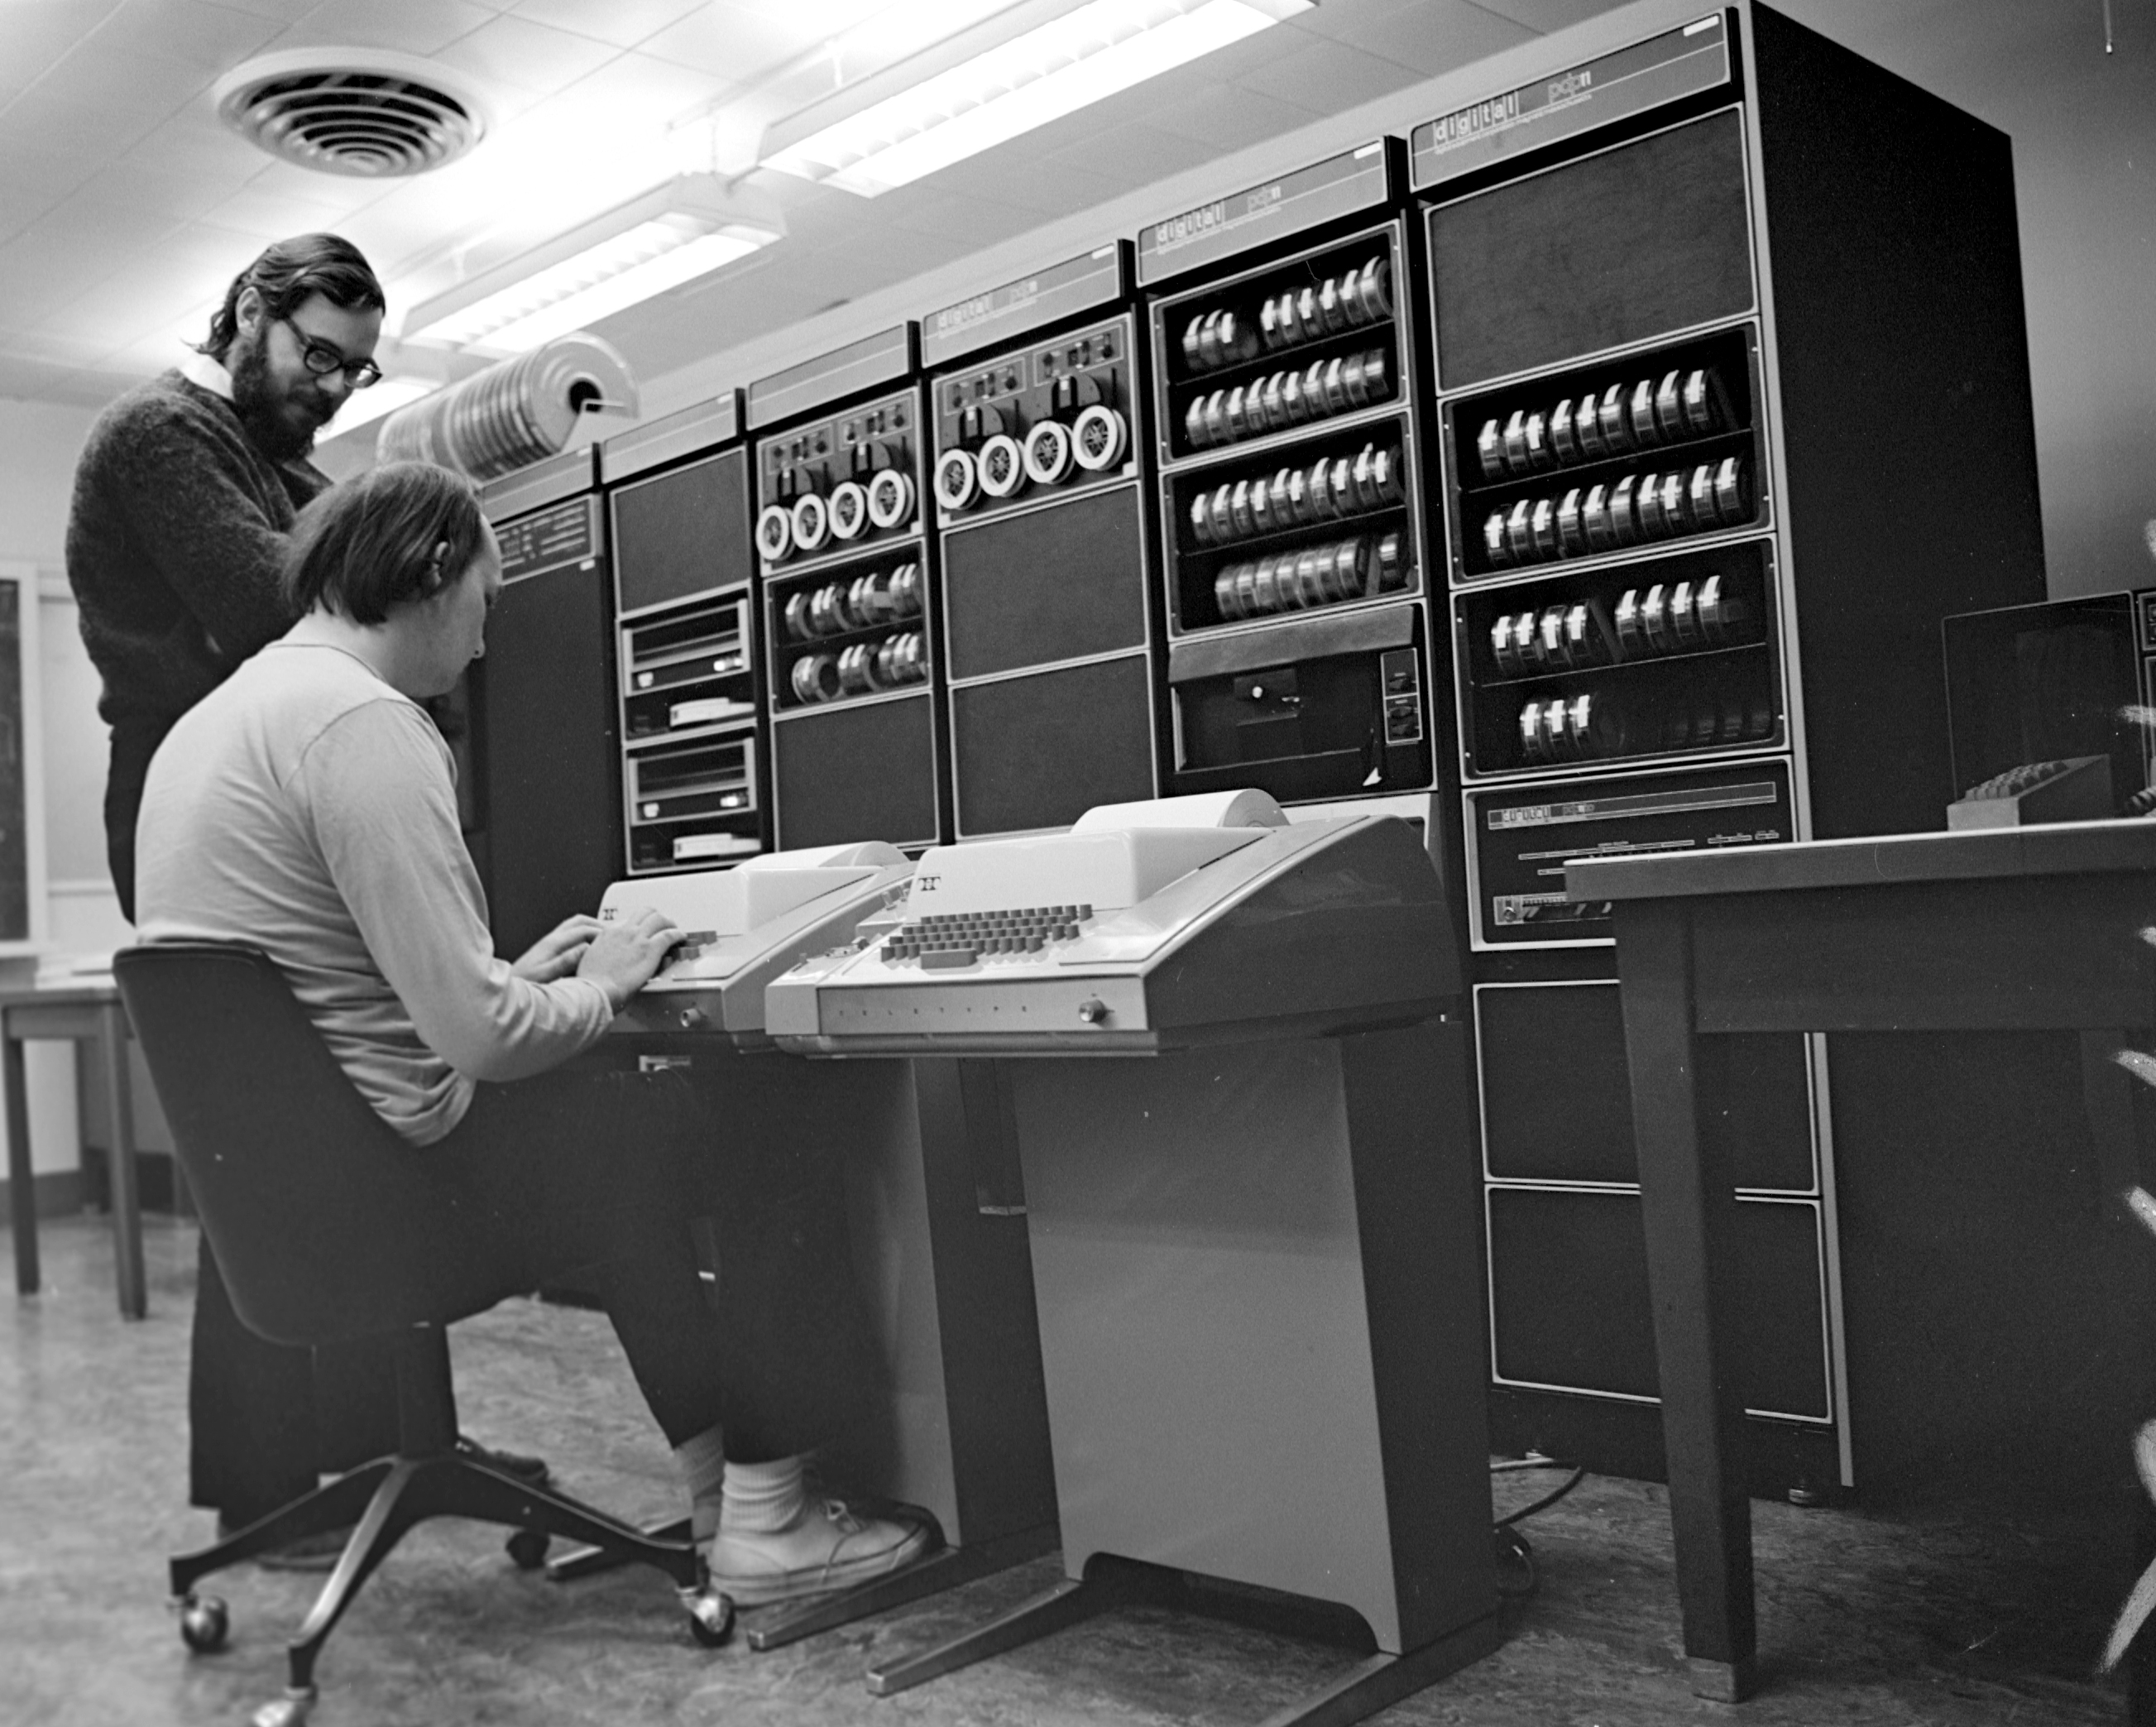
\includegraphics[width=.7\textwidth]{im/Ken_Thompson_(sitting)_and_Dennis_Ritchie_at_PDP-11_(2876612463).jpg}
\end{center}
\footnote{Ken Thompson and Dennis Ritchie on a PDP-11}
\end{frame}
%automate
%demo %%set up 20 files ahead of time
%document
%share
%version
%github
\begin{frame}
  \begin{center}
  \Huge live coding caveat
  \end{center}
\end{frame}

\begin{frame}{Benefits of command line}
\Large
\begin{columns}
\begin{column}{.2\textwidth}
\vspace{.1in}
\end{column}
\begin{column}{.8\textwidth}
\begin{center}
\begin{itemize}
\item Automation
\item Reproducibility
\item Required to run many programs
\end{itemize}
\end{center}
\end{column}
\end{columns}
\end{frame}

\begin{frame}{Benefits of command line}
\begin{center}
\Huge Example
\end{center}
\end{frame}

\begin{frame}{Making it easier}
\begin{center}
\begin{tabular}{rl}
\Large Tab completion & Press \texttt{Tab} once to autocomplete. \\
&Press \texttt{Tab} twice to list potential completions.\\
\Large History & Press \texttt{Up} or \texttt{Down} to view/edit previous commands.\\
\Large man & Type \texttt{man XXX} to get help on command XXX.\\
\Large google & Lots of webpages. Add ``linux'' and/or ''tutorial''\\
\end{tabular}
\end{center}
\end{frame}


\section{Directories}
\framedgraphic{Directories}{im/directories.jpg}
\begin{frame}{Directory shortcuts}
\begin{center}
{\def\arraystretch{1.7}
\begin{tabular}{|c|c|}
\hline
\Large \texttt{.} &The current ``working'' directory\\
\hline
\Large \texttt{..} &The parent directory of the current directory\\
\hline
\Large \texttt{\texttildelow} &Your home directory (different for each user)\\
\hline
%\Large \texttt{/} &The root directory. The very base of the filesystem.  Something like the ``Computer'' directory in Windows.\\
%\hline
\Large \texttt{-} &The last directory\\
\hline
\end{tabular}
}
\end{center}
\end{frame}
%picture of directories
\section{ls}
\begin{frame}
\begin{center}
\Huge ls
\end{center}
\end{frame}
%demo
\section{cd}
\begin{frame}
\begin{center}
\Huge cd
\end{center}
\end{frame}
%demo
\begin{frame}
\begin{center}
\Huge pwd
\end{center}
\end{frame}
\section{mkdir}
\begin{frame}
\begin{center}
\Huge mkdir
\end{center}
\end{frame}

\begin{frame}
  \begin{center}
  \Huge Practice
  \end{center}
\end{frame}

\begin{frame}{What next?}
\Large
\begin{columns}
\begin{column}{.2\textwidth}
\vspace{.1in}
\end{column}
\begin{column}{.8\textwidth}
\begin{center}
\begin{itemize}
\item LinuxCommand.org\\
\item google: software carpentry unix\\
\end{itemize}
\end{center}
\end{column}
\end{columns}

\end{frame}

%\framedgraphic{Experimental setup}{im/pacBio/Methods_2.png}
\end{document}
